%%%%%%%%%%%%%%%%%%%%%%%%%%%%%%%%%%%%%%%%%%%%%%%%%%%%%%%%%%%
% EPFL report package, main thesis file
% Goal: provide formatting for theses and project reports
% Author: Mathias Payer <mathias.payer@epfl.ch>
%
% This work may be distributed and/or modified under the
% conditions of the LaTeX Project Public License, either version 1.3
% of this license or (at your option) any later version.
% The latest version of this license is in
%   http://www.latex-project.org/lppl.txt
%
%%%%%%%%%%%%%%%%%%%%%%%%%%%%%%%%%%%%%%%%%%%%%%%%%%%%%%%%%%%
\documentclass[a4paper,11pt,oneside]{article}
% Options: MScThesis, BScThesis, MScProject, BScProject
\usepackage[MScProject,lablogo]{EPFLreport}
\usepackage{graphicx}
\usepackage{listings}
\graphicspath{ {./figures/} }
\usepackage{xspace}

\title{Semester project on Fuzzing Trusted Execution Environments on COTS Android Devices}
\author{Leonardo Pennino}
\supervisor{Dr. Marcel Busch}
\adviser{Prof. Dr. sc. ETH Mathias Payer}
%\coadviser{Second Adviser}

\newcommand{\sysname}{TEEzz\xspace}

\begin{document}
\maketitle
\makeacks

\begin{abstract}
  The \sysname \cite{TEEzz} tool designed by Dr. Marcel Busch enables effective fuzzing of
Trusted Environment by an automatic inferring of the data and value dependency
obtained by looking at the interactions of the TA.
The main work was focused on fixing
and improving the existing Client Application Library Identification (CAID)
tool by enabling multithreaded computation, creating drivers for Trusted
Application in order to trigger interactions with the TEE, improving the build system of the seed recorder, and generating working recorders
for the device Hikey620.
\end{abstract}


\maketoc

\section{Introduction}
Smartphones leverage the use of a Trusted Execution Environment in order to secure sensitive information, perform sensitive functions and handle Digital Rights Management (\textbf{DRM}). Applications can then use vendor provided interfaces (e.g., ~\cite{HuaweiTrustedCore}) to communicate with the underlying TEE. Applications which reside in the \textbf{ROS} (Rich OS) that connect to the Trusted Application through a vendor defined interface are called \textbf{CA} (i.e., Client Application). Applications that reside in the TEE will be referred to as \textbf{TA} (i.e. Trusted Application). Due to the spread of TEE applications, more vulnerabilities in TAs are being discovered. Vulnerabilities inside TAs are particularly dangerous as they could compromise the security of the whole system. Researching the security of TAs remains a challenge due to the complex stateful interactions, proprietary message passing formats, and the inability to inspect the TEE internal state.
Trusted Applications often store data encrypted in secure memory which is then decrypted only at runtime by the TEE, prohibiting the use of static analysis based vulnerability detection techniques. Dynamic analysis techniques such as fuzzing provide an appealing alternative. The challenges of writing effective fuzzers for Android TAs reside on the absence of source code, and the inability of inspecting the Trusted Environment internal state. Due to these limitations the following techniques are being used: \emph{re-hosting through emulation} or \emph{on-device instrumentation}.
Rehosting the TEE in an emulated environment overcomes
the inaccessibility of the TEE’s internal state. PartEmu~\cite{Harrison2020PARTEMUED} re-hosts Samsung’s proprietary TEE software stacks.
They emulated on a system-on-a-chip (SoC) the TEE and the TAs, which allows them unrestricted access to the TEE internal state.
This approach is limited by the inaccuracy of the emulation process, the required manual effort of reverse engineering and by non-disclosure agreements wanted by industries.
The second approach, on-device fuzzing, mitigates these
limitations and inaccuracies of emulation approaches. However, due to the lack of access to the TEE’s internal state it must fall
back to blackbox fuzzing techniques. While typical fuzzing techniques can analyze the binary, memory, and
executed instructions, an on-device TEE fuzzer must infer bugs from a limited view of the execution.
Blackbox fuzzing is unable to capture and make us of
message semantics required by the TAs for the interactions, making the fuzzing process rather inefficient. This is why new techniques are needed to effectively find vulnerabilities in Trusted Applications.
\subsection{TEEzz}
We present TEEzz, a state and type aware fuzzing framework for TAs running on COTS Android devices.
TEEzz first identifies the TAs
within the TEE and then triggers interactions with
them. During these interactions, TEEzz records the data passed
both into and out of the TEE to automatically reconstruct the
message semantics and value dependencies.
Lastly, this message format, along with the dependencies of
the interaction (i.e.,getting a token from the TEE and then sending it back in a subsequent for authentication), are fed into our fuzzer. The fuzzer
explores the TA while continuously checking for liveness and
monitoring for crashes.
TEEzz automatically generates
memory introspection logic for each parameter type of the
exposed interface. At runtime, we dynamically
instrument this interface, parse the values corresponding to
each type on-the-fly from memory, and save the type-aware
token sequence to disk.
The tasks done in this project are presented in the next sections.
\subsection{Improving library identification}
The tool TEEzz-CAID described in \autoref{sec:teezz-caid}, responsible for CA applications, originally was working only on Huawei and Xiaomi Android devices. It has been rewritten to support any vendor by building and
injecting missing binaries on the phone which are essential for the tool.
Furthermore, the program was sped up by dividing its computation in multiple
threads, and restructured to be more maintainable and able to scale.
\subsection{Writing C++ drivers for closed-source client applications}
A driver for Xiaomi Mlipay as described in \autoref{sub:CDrivers} was developed to trigger interaction with the corresponding TA. This required reverse engineering the ARM64 C++ executable shipped by the vendor.
\subsection{Writing drivers using Java Reflection}
While the previous part focused on writing C++ drivers for closed-source TAs, the next task was focused on writing Java drivers, using Java reflection, for TAs taken from the Android Open Source Project, see \autoref{sub:javaref}.
In particular, we focused on implementing drivers for \emph{Keystore} and \emph{Gatekeeper} able to trigger all available interactions with the corresponding TA.
\subsection{Seed Recorder}
The last part of the project was focused on automating the build process of the Seed Recorder described in \autoref{sub:seedrecorder}.
The seed recording was converted to a docker container able to automatically
download the required Android source code, compile needed libraries, and set up all the
required objects for the recorder to work with. Additionally, due to the changes introduced by Google in Android 8 regarding HAL interfaces ~\cite{HuaweiTrustedCore}, downloading the AOSP code was no longer sufficient for the inference of struct and class types. Work has been done to automatically generate C and C++ from HIDL descriptor files in order to correctly set up the recorder, more in \autoref{sub:HIDL}.

\subsection{Resources}
The project is divided in 3 different repositories:
\begin{itemize}
  \item \href{https://github.com/HexHive/teezz-caid}{https://github.com/HexHive/teezz-caid}
  \item \href{https://github.com/HexHive/teezz-ca-driver}{https://github.com/HexHive/teezz-ca-driver}
  \item \href{https://github.com/HexHive/teezz-introspection}{https://github.com/HexHive/teezz-introspection}
\end{itemize}

%%%%%%%%%%%%%%%%%%%
\section{Library Identification}
\label{sec:teezz-caid}
%%%%%%%%%%%%%%%%%%%
The first goal of the project is to provide a mean to detect which Android
applications or libraries are accessing the Trusted Execution Environments.
TEEzz-CAID is a tool specifically made for this purpose,it scans an Android device and searches for every app or library that is directly or
indirectly calling communicating with the TA.
The tool was able to generate dependency graphs for Xiaomi and Huawei devices, it has now been rewritten to support any vendor. Furthermore, the program was sped up by making use of multiple threads, which made the execution 200\% faster.
The program requires as input
the \emph{main} TEE client API library for the connected device e.g.:\emph{libteec.so} for devices with Arm Cortex-A cores using the TrustZone technology.
The program will then build a graph where on its vertexes we find all the
libraries and consumers that eventually call into the ta which is the root node.
The process is divided in three parts:
downloading binaries, disassembling and finding dependencies.
\subsection{Downloading binaries}
The first part of the process relies in getting all executables, libraries
and VDexs from the device. In order to do so we spawn a shell and we execute
\emph{file} for each one of them. The first problem we faced was that many vendors
do not include all required \emph{Unix binaries} which are needed by the program
such as \emph{file} or \emph{find}.To solve this problem we have statically
compiled those utilities that will be injected into the device if needed.
Another issue is that pulling large amounts of files from android phones is not a fast process, to solve this issue we divide the pulling operation in more threads to improve execution time.

\subsection{Disassembling}
Once the program downloads the required files, we have two different categories
of files and each will be treated differently: \textbf{ELF files},
and \textbf{VDexs}. For ELF files \emph{readelf} is used to get all the libraries
needed by the executable. It will also list libraries loaded dinamycally with \emph{dlopen}
by specifically looking for the \emph{dlopen} or
\emph{hw \textunderscore get\textunderscore module} symbols.
\emph{VDexs} files instead are firstly extracted using vdexExtractor, then
decompiled using jadx. Once that is done a process similar to ELFs is followed,
in particular we look for \emph{System.LoadLibrary} to check which libraries
it is using.
\subsection{Finding Dependencies}
At the end of the before mentioned process, a list of Vdexs and Elfs is obtained, each one with
their own dependencies. The program starts by putting the main CA library given
as input on a stack, then it will scan the built list for every file that has
that library as a dependency. Every match is put on the stack and the previous
item is popped, then recursively repeats the
process until no items remain on the stack. At the end we obtain
a graph with all the found libraries and applications.  Figure~\ref{fig:nexus5x} and Figure~\ref{fig:gs10e} illustrate graphs generated by the tool.
\begin{figure}[!htb]
  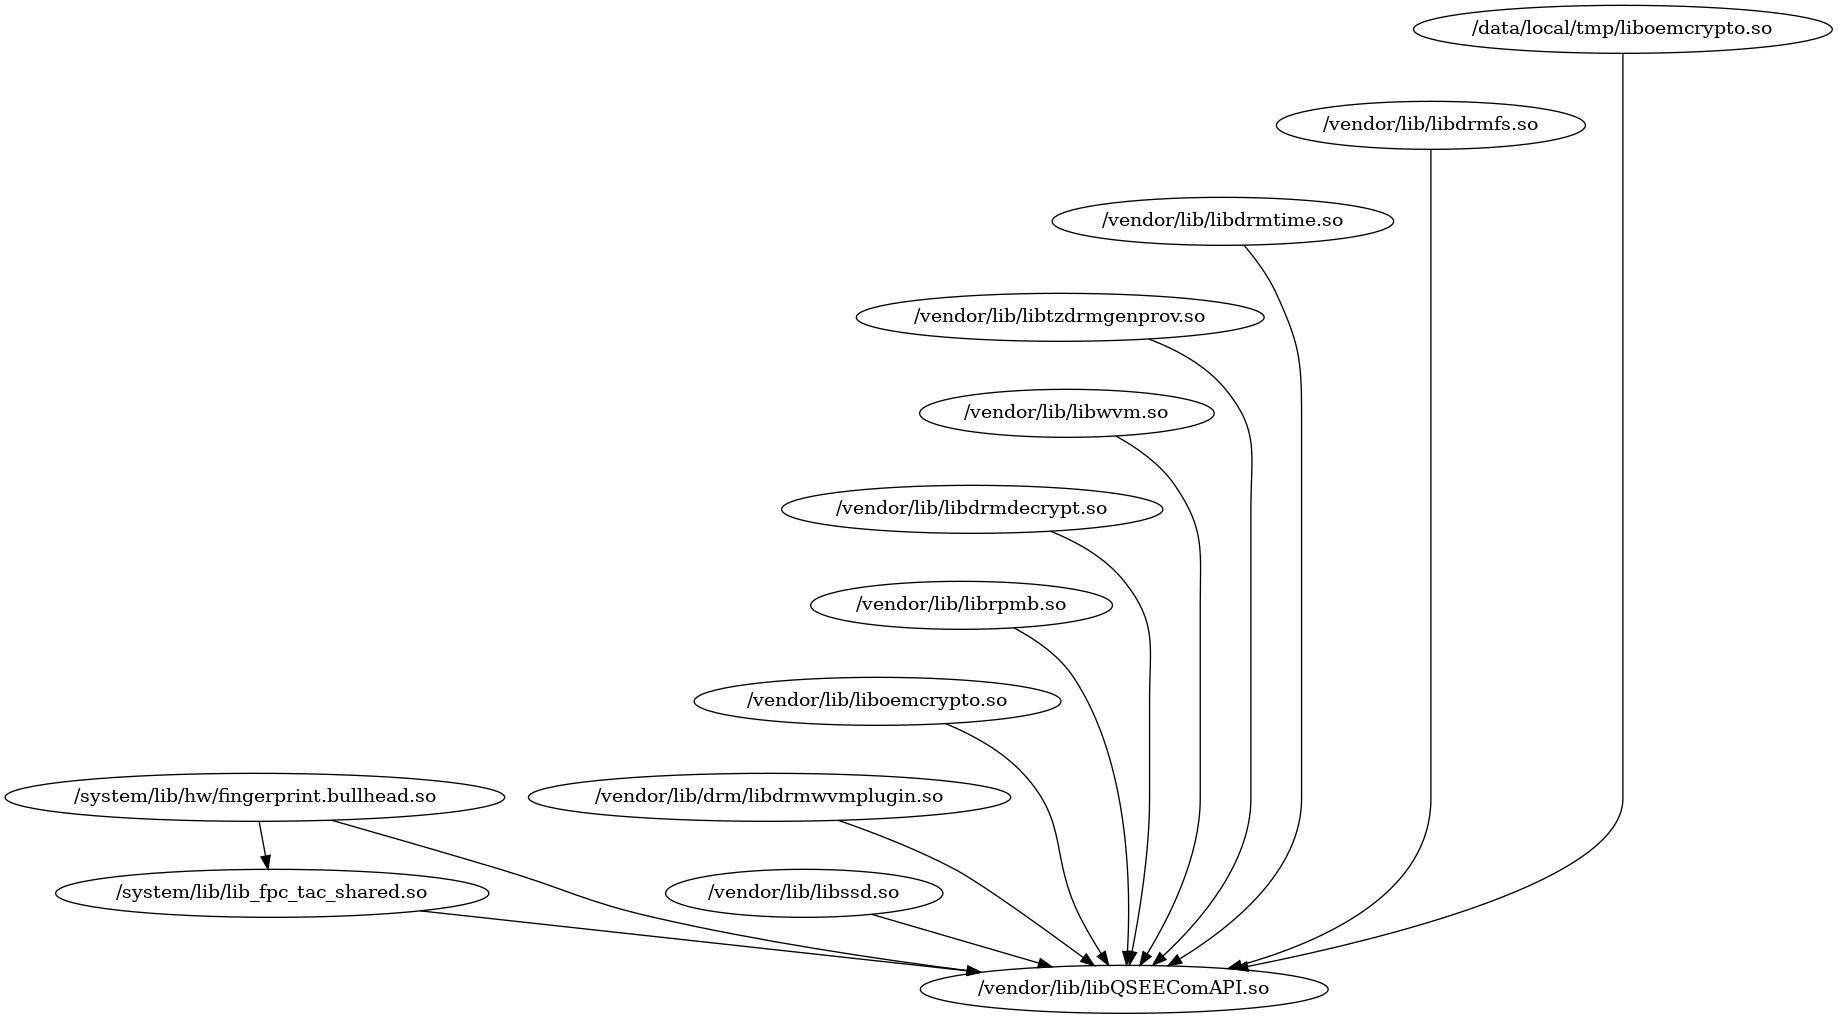
\includegraphics[width=16cm, height=16cm]{figures/nexus5x.png}
  \label{fig:nexus5x}
  \caption{Graph obtained from the device Nexus 5X. As we can see libQSEECOMAPI.so is the main library for communicating with the TEE. All other libraries add abstraction layers on top of it.}
\end{figure}
\begin{figure}[!htb]
  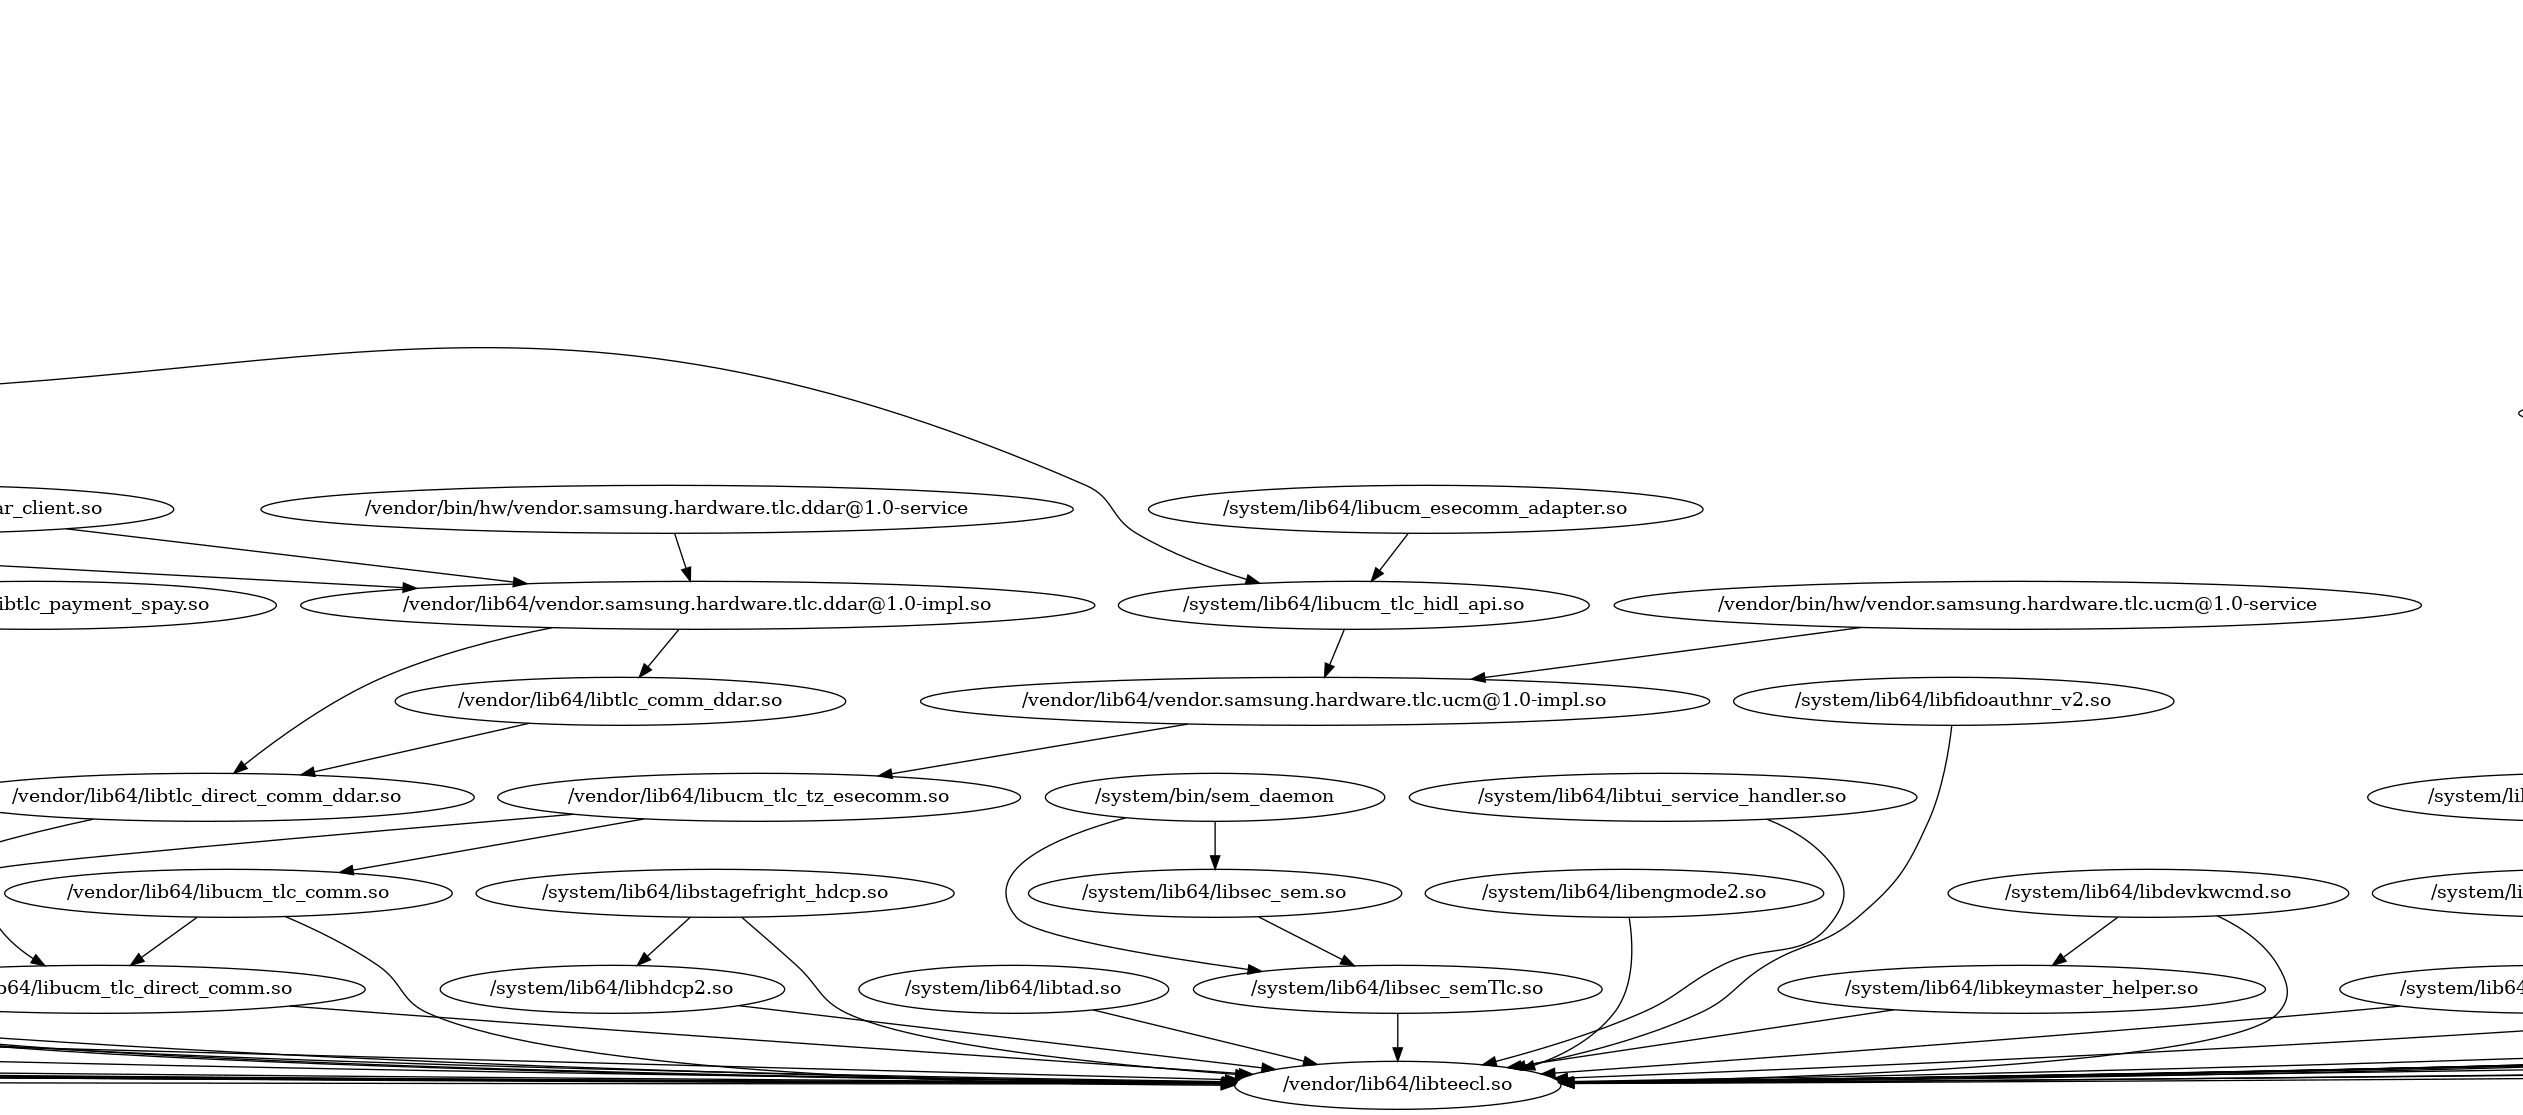
\includegraphics[width=16cm, height=16cm]{figures/gs10e.png}
  \label{fig:gs10e}
  \caption{A cropped graph obtained from the device Galaxy S10e. This pictures shows a much interesting results as we can clearly see how different abstraction layers are stacked on top of each other by the vendor.}
\end{figure}
\paragraph{Drawbacks of TEEzz-CAID}
Due to the errors that can arise from Java decompilation, we are not always able to detect all Vdexs which are using a specific library. Furthermore, in order to find the library used with \emph{dlopen}
and \emph{hw \textunderscore get\textunderscore module},we run \emph{strings} on the target binary and grep for specific libraries. This means that if there are name obfuscation in process when loading the library (e.g., xoring the library name with a key at runtime) we cannot correctly identify them. Due to these issues, the graphs provided by the program can not be considered \textbf{complete} until some other mechanisms are added.


%%%%%%%%%%%%%%%%
\section{Triggering interactions with the TA: Drivers}
%%%%%%%%%%%%%%%%
Since \sysname relies on the seeds generated by interactions
with the TA, we need a method to trigger interactions at our will.
Interaction with the TAs can be achieved in two ways:
manual interaction with the device, or by calling functions in CAs that will result in a request to the TEE. Programs able to call CA functions are called \textbf{drivers}. We have managed to successfully implement drivers for \emph{Gatekeeper} and \emph{Keystore} that can call every function defined in their respective interface.
We have also implemented a prototype driver for Xiaomi Mlipay able to call one function of the CA, more on that in \autoref{sub:CDriver}.
\subsection{Manual Interaction}
Manual interactions with the Trusted Execution Environment happen when
specific events occur that require an interaction with the Secure World e.g., changing lock-screen code on an Android phone triggers a request
to the \emph{Gatekeeper} TA in order to submit and approve the changes. Doing this effort
manually each time requires a lot of time and makes our fuzzing very inefficient.
The first approach was to emulate touches on the Android phone using a
program that we designed to trigger the touches as fast as possible.
This solution was fast to implement and correctly working however it
took around 3 minutes for some specific interactions.
Certain Android devices such as Huawei in order to
remove the lock-screen code, needed to trigger a particular interaction in the
\emph{Gatekeeper}, require 5 wrong tries, with 30 seconds delay between
each other, thus the whole process took 3 minutes each time.
\subsection{Interactions using Java Reflection}
\label{sub:javaref}
Seeing these drawbacks, we opted
for another path. We found a way to trigger interactions using Java
Reflection. We first build a
Java program which hooks into Android Java classes such as \emph{Gatekeeper}
via \textbf{Class.forName}, then we can trigger methods or create objects.
After having built our Java file we \textbf{dex} it and inject into our test device and
run it via \emph{app\textunderscore process}. An example driver that uses Java Reflection is given in \autoref{lst:keystoreCAjava}. This approach does not have the
drawbacks of
the one discussed before, however not every Client Application has a Java
callable interface, hence why this approach cannot be used in all scenarios. Furthermore, we are only able to call functions exported from the Java interface, which means that there might be functions of the TAs that we are not covering.
\begin{lstlisting}[label= {lst:keystoreCAjava}, language=Java, caption=Example driver for Keystore using Java Reflection]
public KeystoreClient() {
      Class IKeystoreService = Class.forName(
      "android.security.IKeystoreService");
      Class stub = IKeystoreService.getDeclaredClasses()[0];
      Method mAsInterface = stub.getDeclaredMethods()[0];
      //Final object able to call binder
      oKeystoreService = mAsInterface.invoke(null, getKeystoreBinder());
      //now we can access the methods
      mReset = oKeystoreService.getClass().getDeclaredMethod("reset");
      mGet = oKeystoreService.getClass().
      getDeclaredMethod("get", String.class, int.class);
      // we can call methods like this
      mGet.invoke(oKeystoreService,...params);
    }
\end{lstlisting}
\subsection{Interaction with custom C/C++ drivers}
\label{sub:CDriver}
To cover also applications which do not communicate via Java interfaces, we build C or C++ drivers by making use of \emph{dlopen}.
Xiaomi's \emph{mlipay} library
which is used for payments, is one such example. We have to build a driver able to construct the MLIPAY object and call into its functions. In order to
build such a driver, first we have to reverse engineer the library to
understand its functionalities, the functions and objects it exports, the value dependencies and the required structs and parameters. Once we have that sorted, we create a handle to the \emph{shared object} and
attach it using \emph{dlopen}. Listing~\ref{lst:MlipayCA} contains example code of such a driver.
We have managed to write a driver for one of MLIPAY's functions by calculating the offset in the Virtual Table and manually jumping at that address.
An example is provided in \autoref{lst:MlipayCA}.
The manual offset jump calculation can be automated if we reverse engineer the object struct, construct it in memory with the exact sizes and paddings and then use its function pointers to jump..
However, the development of drivers for C++ binaries requires a lot of manual effort. Furthermore, reversing C++ binaries is always a challenge due to how they are compiled. In addition, hooking into C++ object is also more difficult than C objects as it requires to find a way to call the constructor and get a reference to the object, and also figuring out the object layout in memory to jump into the correct code regions.
\begin{lstlisting}[language=C++, label={lst:MlipayCA}, caption= Example driver for mlipay using dlopen]
int main(int argc, char **argv) {
  void *handle = dlopen("libmlipay.so", RTLD_NOW | RTLD_GLOBAL);
  if (handle == NULL) {
    printf("Error opening handle to libmlipay.so");
    return -1;
  }
  void *(*fn)(void) = NULL;
  void *(*constructor)(void) = NULL;
  void *(*get_key_version)(void) = NULL;
  printf("Created handle \n");
  *(void **)(&fn) = dlsym(handle, "HIDL_FETCH_IMlipayService");
  if (fn != NULL) {
    printf("Calling fn\n");
    void **obj = (void **)(*fn)();
    void **vtable = (void **)*obj;
    *(void **)(&constructor) = (void **)*(vtable);
    *(void **)(&get_key_version) = (void **)*(vtable + 0xe);
    //The address above was obtained via reverse engineering
    (*get_key_version)(); // Calling our target function
  }
}
\end{lstlisting}

%%%%%%%%%%%%%%%%%%%%%%%%

%%%%%%%%%%%%%%%%%%%%
\section{Seed Recording}
\label{sub:seedrecorder}
%%%%%%%%%%%%%%%%%%%%
The last part of the project focused on improving, making the seed
recorder portable, easily reproducible and adaptable to various devices.
The seed recorder is the part of the project that is
responsible to create type aware seeds for the fuzzer.
The recording works at different abstraction levels:
\textbf{IOCTL} and the \textbf{Hardware Abstraction Layer}.
It uses Frida to dinamycally instrument code on the target device to execute arbitrary code allowing the inspection and dumping of the memory.
For the IOCTL layer
layer we just need to hook into the \emph{ioctl} system
call and dump the data sent.
The HAL layer is just above the IOCTL and this contains struct definitions, types and value dependencies.
The seeds that need to be generated from HAL and IOCTL are very different. More work is needed for the HAL to correctly identify the data that the
application passes to the TEE.
The seed recorder consists of the following parts: the \textbf{Interceptor}, \textbf{Generator}, \textbf{FridaDumper}, \textbf{HalDumper} and \textbf{DualRecorder}.
\subsection{Interceptor}
The role of the interceptor is to attach the frida debugger to the function calls we want to look into.
The interceptor takes as parameter a json file describing
the interface's functions and how to locate them, either via symbols if the binary is non stripped or by offset.
It can either attach by symbol name or function offset.
After attaching to a function it automatically dumps the incoming and outgoing parameters.
\label{sec:Gendumper}
\subsection{Gendumper}
The gendumper takes as input a C/C++ file and a struct or class and dumps the js code which will be then used by frida, with type and state awareness. In order to correctly parse the input file it makes use of clang to build an
AST, which it explores to find the definition for each type and function of the input symbol. To work as
expected, it requires all C / C++ headers that the input file uses. To make the software portable and readaptable, the download and compilation of required libraries has to be automated. The docker container included in the seed recorder contains \emph{Makefiles} for different devices that automatically download and compile the needed libraries from the AOSP and generate the header files required by the gendumper.
\subsection{FridaDumper}
The FridaDumper instruments the Client Application in order to hook into \emph{ioctl} and dump the data flow.
\subsection{HalDumper}
The HalDumper takes as input the javascript files generated by the GenDumper and a service to hook into.
It then attaches frida and instruments the binary to
dump function calls, incoming and outgoing parameters for each function contained in the javascript file.
\subsection{Dual Recorder}
The dual recorder is the final step of the project, it combines both the HalDumper and the Frida Dumper into one unique program which is able to generate both seeds that will then be used by the fuzzer.

\begin{lstlisting}[language=bash , caption=Example of seeds recorded for Keystore on Hikey620]

exportKey_10000/onenter:
appData
clientId
exportFormat
keyBlob

exportKey_10000/onleave:
appData
clientId
exportFormat
keyBlob

finish_1000/onenter:
inParams
input
operationHandle
signature

finish_1000/onleave:
inParams
input
operationHandle
signature

importKey_13345/onenter:
keyData
keyFormat
params

importKey_13345/onleave:
keyData
keyFormat
params

update_15005/onenter:
inParams
input
operationHandle

update_15005/onleave:
inParams
input
operationHandle

\end{lstlisting}
\section{Challenges}
During this project many challenges had to be faced, we will try to give a brief summary of them in chronological order.
\subsection{On writing handles for C++ libraries}
Writing the handle for the MLipay library has proved
to be a difficult challenge because of how C++ is compiled. After research and with the help of Marcel and the HexHive group I managed to
reverse a small part of the binary and to locate the function pointers on the Virtual Table created which then I used to call into the library's code.
\subsection{Understanding Android Stub and HIDL Java}
Android Stub interfaces and how and HIDL interface
is called from java was not as straightforward as I
thought it would be. It took a lot of reading through
the android code base in order to build a driver with
the same interface as the library it calls underneath.
I wanted the driver to have the same interface so that testing and running would be easy and clear.
\subsection{Automatic code download from Google Code Source and HIDL Generation}
\label{sub:HIDL}
Since Gendumper needs all the libraries that the
headers supplied require, an automatic download of
the android source was needed. This was a problem for
two reasons: firstly because the android master branch always changes and it may include breaking changes for
older android versions e.g.: the android build system changes again, and second because of Google switching from C headers to HIDL files. Automatic generation of header files from HIDL definitions was achieved via downloading the code from a specific branch or a specific commit. The hardest challenge for gendumper was that it also required the exact clang arguments and headers that were used for a specific version of the library. To get the gendumper to work on optee I had to
clone the whole android source and manually inspect the build process to figure out the exact libraries and clang arguments.
%%%%%%%%%%%%%%%%%%%%
\section{Conclusion}
%%%%%%%%%%%%%%%%%%%%
The project at its current state is perfectly able to
identify and collect all the Client Application from a device,
provide drivers for Android's Keymaster and Gatekeeper Client Applications and to record interaction for the device Hikey620. Adding support to other devices for these 2 CA is straightforward as the project generates the code automatically, support for other libraries can be added by following the guides available on the repository. The future of the project relies on adding support for other libraries and devices.

\cleardoublepage
\phantomsection
\addcontentsline{toc}{section}{Bibliography}
\printbibliography

% Appendices are optional
% \appendix
% %%%%%%%%%%%%%%%%%%%%%%%%%%%%%%%%%%%%%%
% \section{How to make a transmogrifier}
% %%%%%%%%%%%%%%%%%%%%%%%%%%%%%%%%%%%%%%
%
% In case you ever need an (optional) appendix.
%
% You need the following items:
% \begin{itemize}
% \item A box
% \item Crayons
% \item A self-aware 5-year old
% \end{itemize}

\end{document}
